\documentclass{article}


\usepackage{arxiv}

\usepackage[utf8]{inputenc} % allow utf-8 input
\usepackage[T1]{fontenc}    % use 8-bit T1 fonts
\usepackage{hyperref}       % hyperlinks
\usepackage{url}            % simple URL typesetting
\usepackage{booktabs}       % professional-quality tables
\usepackage{amsfonts}       % blackboard math symbols
\usepackage{nicefrac}       % compact symbols for 1/2, etc.
\usepackage{microtype}      % microtypography
\usepackage{lipsum}
\usepackage{graphicx}
\usepackage{subcaption}
\usepackage[margin=1in]{geometry}
\usepackage{amsmath}
\usepackage[spanish]{babel}
\usepackage{float}
\usepackage{adjustbox}
\usepackage{placeins}
\graphicspath{ {./images/} }
\renewcommand{\refname}{Referencias}


\title{TP 3 - Simulación de Modelos: MM1 e Inventario.}


\author{
 Aldana Risso Patrón \\
  Universidad Tecnológica Nacional - FRRO \\
  Zeballos 1341, S2000, Argentina \\
  \texttt{rissopatronaldana7@gmail.com} \\
   \And
 Ignacio Fierro \\
  Universidad Tecnológica Nacional - FRRO \\
  Zeballos 1341, S2000, Argentina \\
  \texttt{nachofier@gmail.com} \\
  \And
 Lucía Gelmetti \\
  Universidad Tecnológica Nacional - FRRO \\
  Zeballos 1341, S2000, Argentina \\
  \texttt{luligelmetti@gmail.com} \\
  \And
 Juan Cruz Bonanno \\
  Universidad Tecnológica Nacional - FRRO \\
  Zeballos 1341, S2000, Argentina \\
  \texttt{bonanno2340@gmail.com} \\
  \And
 Franco Reggiardo Chuglar \\
  Universidad Tecnológica Nacional - FRRO\\
  Zeballos 1341, S2000, Argentina \\
  \texttt{francoreggiardo15@gmail.com} \\
  \And
 Marcos Oldani \\
  Universidad Tecnológica Nacional - FRRO \\
  Zeballos 1341, S2000, Argentina \\
  \texttt{marcosoldani1360@gmail.com} \\
}

\begin{document}
\maketitle
\begin{abstract}
Este trabajo práctico tiene como objetivo estudiar, mediante simulación, el comportamiento de dos modelos clásicos: el modelo de colas \( M/M/1 \) y un modelo de inventario. Se analizarán diferentes métricas de rendimiento bajo diversas condiciones experimentales y se compararán los resultados obtenidos mediante simulación en Python, el software AnyLogic y los valores teóricos esperados.
\end{abstract}

\section{Introducción}
En el ámbito de la investigación operativa y la gestión de sistemas, la simulación emerge como una herramienta poderosa para analizar y comprender el comportamiento de sistemas complejos que, de otro modo, serían difíciles de modelar analíticamente. Este trabajo se enfoca en la simulación de dos modelos : el modelo de colas M/M/1 y un modelo de inventario, fundamentales para la optimización de procesos en diversos sectores, desde la manufactura y la logística hasta los servicios y las telecomunicaciones.

\section{Teoría de Colas}
Una \textbf{cola} se forma frecuentemente cuando una serie de \textit{clientes} solicita un \textit{servicio}, y tanto el servicio como los clientes tienen un comportamiento probabilístico. La primera aplicación de la teoría de colas se atribuye al matemático danés Erlang, quien en 1909 utilizó estos conceptos para calcular el tamaño de las centralitas telefónicas.

La teoría de colas es una disciplina de la Investigación Operativa que se enfoca en proponer modelos para la gestión eficiente de líneas de espera. Una \textbf{línea de espera} es una fila compuesta por uno o varios clientes que esperan para recibir un servicio. Estos clientes pueden ser personas, objetos, máquinas que requieren mantenimiento, contenedores de mercancías para ser embarcados, elementos de inventario para ser utilizados, entre otros.

Una línea de espera se forma debido a un desequilibrio temporal entre la demanda de un servicio y la capacidad del sistema para gestionarlo. Los modelos de líneas de espera son muy útiles para determinar cómo operar un sistema de colas de manera más eficaz, ya que permiten encontrar un balance adecuado entre el costo del servicio y el tiempo de espera. Proporcionar demasiada capacidad de servicio implica costos excesivos, mientras que una capacidad insuficiente resulta en esperas prolongadas con consecuencias negativas.

Aunque cada situación específica tiene características diferentes, existen cuatro elementos comunes a toda Línea de Espera:
\begin{itemize}
    \item Una población de clientes que genera clientes potenciales.

    \item Una línea o fila de espera formada por los clientes.

    \item La instalación del servicio, formada por una persona (o un equipo), una máquina (o grupo de máquinas) que se requiere para proveer el servicio que el cliente solicita.

    \item Una regla de prioridad para seleccionar al siguiente cliente que será atendido por la instalación de servicio
\end{itemize}

El término ``cliente'' se utiliza en un sentido general, pudiendo ser una persona, piezas esperando su turno para ser procesadas, una lista de trabajo esperando para ser impresas en una impresora de red, etc.

Básicamente la mayoría de los modelos de colas consiste: Los \textbf{clientes} que requieren un \textbf{servicio} se generan en el tiempo en una \textbf{fuente de arribo}, después entran al \textit{sistema} y se unen a una cola. 

En determinado momento se selecciona a un cliente de la cola para proporcionarle el servicio mediante alguna regla conocida como \textbf{disciplina de la cola}. Se lleva a cabo el servicio que el cliente requiere mediante un \textbf{Mecanismo de servicio}, y después el cliente sale del sistema de colas.
\subsection{Tipos de Sistemas de Cola}
Los sistemas de cola se pueden diferenciar teniendo en cuenta el número de arribo, salidas, colas y servidores. As1í tenemos los siguientes casos:
\begin{itemize}
    \item \textbf{Una cola y un servidor:}
    \begin{figure}[H]
        \centering
        \includegraphics[width=0.5\linewidth]{imagenes/cola-servidor.png}
    \end{figure}

    \item \textbf{Una cola y múltiples servidores:}
    \begin{figure}[H]
        \centering
        \includegraphics[width=0.5\linewidth]{imagenes/cola_mult-serv.jpg}
    \end{figure}

    \item \textbf{Varias colas y múltiples servidores:}
    \begin{figure}[H]
        \centering
        \includegraphics[width=0.5\linewidth]{imagenes/mult-colas_mult-serv.png}
    \end{figure}

    \item \textbf{Una cola y servidores secuenciales:}
    \begin{figure}[H]
        \centering
        \includegraphics[width=0.7\linewidth]{imagenes/cola-servSec.png}
    \end{figure}
\end{itemize}

\subsection{Características de los Sistemas de Cola}
Un sistema de colas se describe adecuadamente con seis características:
\begin{itemize}
    \item \textbf{Fuente de arribo de clientes}:  En situaciones de colas habituales, el arribo de clientes es estocástico, esto es, depende de una variable aleatoria, con lo que se necesita conocer la distribución probabilística entre dos arribos sucesivos de clientes. La fuente de arribo puede variar con el tiempo, cuando se mantiene constante se dice \textit{estacionaria}, si varía (por ejemplo, con las horas del día) se llama \textit{no estacionaria}.

    Pueden contemplarse distintas situaciones: Clientes que llegan independiente o simultáneamente (llegan lotes), en este último caso hay que definir su distribución probabilística.  Clientes que abandonan la cola por ser demasiado larga o que tras esperar mucho abandonan.
    
    \item \textbf{Patrón de servicio de servidores}: Pueden presentar un tiempo de servicio variable, en cuyo caso hay que asociar una función de probabilidad. Pueden atender en lotes o de modo individual. El tiempo de servicio puede variar con el número de clientes en la cola, trabajando más rápido o más lento, en este caso se conoce como \textit{patrones de servicio dependientes}. El patrón de servicio puede ser \textit{no estacionario} variando con el tiempo transcurrido.
    
    \item \textbf{Disciplina de cola}: Es la regla en el orden que se van a seleccionar los clientes que se encuentran a la espera de ser atendidos en la cola, existen varias reglas, entre las más comunes se pueden encontrar:
        \begin{itemize}
            \item \textit{FIFO (first in first out)}: Se atiende al cliente en el orden que llegan a la cola, el primero en llegar será el primero en ser atendido. En los modelos básicos de colas se supone como normal la disciplina de primero en entrar, primero en salir, a menos que se establezca de otra manera.

            \item  \textit{LIFO (last in first out)}: Consiste en atender primero al que ha llegado de último, también se le conoce como ``pila''.

            \item   \textit{RSS (random selection of service)}: Se selecciona a los clientes de una cola de forma aleatoria, con algún procedimiento de prioridad o algún otra preclasificación.

            \item \textit{Processor Sharing}: Todos los clientes perimentan con eficacia el mismo retraso, ya que comparten entre todos los clientes de la cola la capacidad del sistema atendiendo a todos por igual.
        \end{itemize}
    
    \item \textbf{Capacidad del sistema}: Es el número máximo de clientes que pueden estar dentro del sistema haciendo cola antes de ser atendidos para recibir el servicio, al igual que la fuente de arribo este número puede ser finito o infinito.
    
    \item \textbf{Número de canales de servicio}: Es preferible utilizar sistemas multiservicios con una única línea de espera para todos que con una cola por servidor. Al hablar de canales de servicio paralelo se trata generalmente de una cola que alimenta a varios servidores.
    
    \item \textbf{Número de etapas de servicio}: Puede ser unietapa o multietapa, en este último el cliente puede pasar por un número de etapas mayor que uno. En algunos sistemas multietapa se admite la vuelta atrás o reciclado, modo habitual en sistemas productivos como controles de calidad y reprocesos.
\end{itemize}

\section{Modelos de Colas Simples}
\subsection{Modelo M/M/1}

El modelo M/M/1 es la base de la teoría de colas, representando un sistema simple con una única cola, un único servidor, arribos que siguen una distribución de exponencial y tiempos de servicio que se distribuyen exponencialmente. La simulación de este modelo no solo permite validar las fórmulas analíticas que describen su comportamiento en estado estacionario, sino que también ofrece una visión invaluable de su dinámica transitoria, es decir, cómo el sistema se comporta desde que inicia hasta que alcanza un equilibrio. Comprender estas dinámicas es crucial para el diseño y la gestión de sistemas donde la espera es una parte inherente del proceso, como centros de llamadas, estaciones de servicio o líneas de producción.

El modelo \( M/M/1 \) se caracteriza por:

\begin{itemize}
    \item Arribos según un proceso de Poisson con tasa \( \lambda \) (clientes por unidad de tiempo).
    \item Tiempos de servicio distribuidos exponencialmente con tasa \( \mu \).
    \item Un solo servidor.
    \item Cola infinita o de tamaño limitado (según variante).
\end{itemize}

\subsubsection*{Métricas de rendimiento}

Para el sistema con cola infinita y en estado estable (\( \rho = \lambda / \mu < 1 \)):

\begin{itemize}
    \item Promedio de clientes en el sistema: \( L = \frac{\rho}{1 - \rho} \)
    \item Promedio de clientes en la cola: \( L_q = \frac{\rho^2}{1 - \rho} \)
    \item Tiempo promedio en el sistema: \( W = \frac{1}{\mu - \lambda} \)
    \item Tiempo promedio en la cola: \( W_q = \frac{\lambda}{\mu(\mu - \lambda)} \)
    \item Utilización del servidor: \( \rho = \frac{\lambda}{\mu} \)
    \item Probabilidad de encontrar \( n \) clientes en la cola: \( P_n = (1 - \rho)\rho^n \)
    \item Probabilidad de denegación de servicio para cola finita de tamaño \( K \):
    \[
        P_{denegación} = \frac{(1 - \rho)\rho^K}{1 - \rho^{K+1}}
    \]
\end{itemize}

\subsubsection*{Experimentos propuestos}

Se evaluarán diferentes valores de \( \lambda \) (25\%, 50\%, 75\%, 100\%, 125\% de \( \mu \)), con un mínimo de 10 corridas por experimento.

\subsubsection{Planteamiento del Problema}
En este trabajo se analiza un sistema de cola de un solo servidor (ver Figura \ref{fig:cola-unico}) en el cual los tiempos entre arribos \(A_1, A_2, \ldots\) son variables aleatorias independientes e idénticamente distribuidas (IID), lo que significa que los tiempos entre arribos tienen la misma distribución de probabilidad. Un cliente que llega y encuentra al servidor desocupado entra inmediatamente en servicio, y los tiempos de servicio \(S_1, S_2, \ldots\) de los clientes sucesivos son variables aleatorias IID, independientes de los tiempos entre arribos. Un cliente que llega y encuentra al servidor ocupado se une al final de una única cola. Al finalizar el servicio de un cliente, el servidor selecciona a un cliente de la cola (si hay alguno) siguiendo el principio FIFO (primero en entrar, primero en salir).
\begin{figure}[H]
    \centering
    \includegraphics[width=0.2\linewidth]{imagenes/cola-unico-ser.png}
    \caption{Sistema de colas de servidor único}
    \label{fig:cola-unico}
\end{figure}








\vspace{1em}

\subsection{Modelo de Inventario}
La gestión de inventarios es un componente crítico de la cadena de suministro, cuyo objetivo es equilibrar la disponibilidad de productos con los costos asociados a su almacenamiento. Un modelo de inventario busca determinar las políticas óptimas para reordenar y mantener existencias, minimizando costos de mantenimiento, costos de pedido y costos de escasez. A través de la simulación, podemos explorar cómo diferentes políticas de inventario impactan en estos costos bajo condiciones variables de demanda y suministro, lo que permite identificar estrategias robustas para asegurar la eficiencia operativa y la satisfacción del cliente.

Debido a la incertidumbre en la demanda y el tiempo de entrega de los pedidos (lead time), la simulación es una herramienta muy útil para analizar políticas de inventario y tomar decisiones más informadas.

\begin{itemize}
    \item Costo de orden (\( C_o \)): cada vez que se realiza un pedido.
    \item Costo de mantenimiento (\( C_h \)): por unidad almacenada por unidad de tiempo.
    \item Costo de faltante (\( C_s \)): penalización por no satisfacer la demanda.
\end{itemize}

\subsubsection*{Modelo básico de revisión periódica (s, S)}

Un modelo común es el de revisión periódica, donde se hace un pedido para llevar el inventario a un nivel \( S \) cuando baja de un umbral \( s \). La demanda es aleatoria y puede seguir, por ejemplo, una distribución normal o Poisson.

\subsubsection*{Métricas de rendimiento}

\begin{itemize}
    \item Costo total: 
    \[
        C_{total} = C_o + C_h + C_s
    \]
\end{itemize}

Los parámetros del modelo serán definidos por los estudiantes y justificados en base al contexto elegido.

\vspace{1em}

\section{Comparación de Resultados}
Se realizará la comparación entre:
\begin{itemize}
    \item Resultados teóricos (basados en fórmulas).
    \item Resultados de simulación con Python.
    \item Resultados obtenidos con AnyLogic.
\end{itemize}

\section{Modelo M/M/1}

\subsection{Valor teórico esperado}}
Como dijimos anteriormente, este modelo se caracteriza por tener una única línea de espera con capacidad finita \( K \), una tasa de arribo \( \lambda \), y una tasa de servicio \( \mu \), asumiendo una política de atención tipo FIFO (First In, First Out).

Uno de los parámetros más relevantes es el factor de utilización del servidor, definido como \( \rho = \lambda / \mu \). A partir de este valor, se pueden deducir distintas métricas esperadas:

- La probabilidad de que el sistema esté lleno (y por lo tanto un arribo sea rechazado), denotada como \( P_K \), depende de si el sistema está en estado estable (\( \rho \ne 1 \)). Se calcula mediante:

\[
P_0 = \frac{1 - \rho}{1 - \rho^{K+1}}, \quad \text{y} \quad P_K = P_0 \cdot \rho^K
\]

- El número promedio de clientes en el sistema, \( L \), y en la cola, \( L_q \), también pueden calcularse en función de \( \rho \), \( K \) y \( P_0 \), usando:

\[
L = \sum_{n=0}^{K} n \cdot P_n, \quad \text{donde} \quad P_n = P_0 \cdot \rho^n
\]

- Los tiempos promedio en el sistema y en la cola (\( W \) y \( W_q \)) se obtienen aplicando la ley de Little:

\[
W = \frac{L}{\lambda_{\text{efectiva}}}, \quad W_q = \frac{L_q}{\lambda_{\text{efectiva}}}
\]

donde \( \lambda_{\text{efectiva}} = \lambda \cdot (1 - P_K) \) representa la tasa de arribos que realmente ingresan al sistema (ya que algunas son rechazadas).

Estos valores sirven como referencia teórica para validar la precisión de los resultados obtenidos por simulación, en especial cuando el número de corridas y el tiempo de simulación son suficientemente grandes como para aproximarse al comportamiento estacionario.


\subsection{En Python}
Para analizar el comportamiento del sistema de colas \( M/M/1/K \), se desarrolló una simulación en lenguaje Python utilizando la biblioteca \texttt{SimPy}, que permite modelar eventos discretos en el tiempo. El sistema considerado representa un único servidor con arribos y tiempos de servicio que siguen distribuciones exponenciales, y una cola de capacidad finita \( K \). En caso de que el sistema esté lleno (es decir, haya un cliente siendo atendido y \( K \) en espera), los nuevos arribos son rechazados.

El código implementa este modelo y permite parametrizar la tasa de arribo (\( \lambda \)), la tasa de servicio (\( \mu \)), la capacidad de la cola (\( K \)) y el tiempo total de simulación, todo a través de argumentos por línea de comandos. Por ejemplo, un posible conjunto de parámetros de entrada sería: \texttt{-a 0.25 -s 1.0 -k 50 -t 1000}, lo que representa una tasa de arribo del 25\% de la capacidad del servidor, con una cola máxima de 50 clientes y una simulación de duración 1000 unidades de tiempo.

El programa realiza un total de 10 corridas independientes para capturar la variabilidad estocástica del sistema. En cada corrida se registran métricas fundamentales tales como la probabilidad de bloqueo (cuando un arribo es rechazado por falta de espacio), el promedio de clientes en el sistema (\( L \)), el promedio de clientes en la cola (\( L_q \)), el tiempo promedio que un cliente pasa en el sistema (\( W \)) y en la cola (\( W_q \)), así como la utilización del servidor. Además, se calculan distribuciones de probabilidad del número de clientes en cola y se realiza un muestreo periódico de su longitud a lo largo del tiempo.

Guardamos los resultados de cada corrida en un archivo \texttt{CSV}.

\subsubsection{Graficas para las distintas tasas de arribo:}
1- Cola vs tiempo: con capacidad de cola infinita ( K = \infty)

    \begin{figure}[h!]
        \centering
        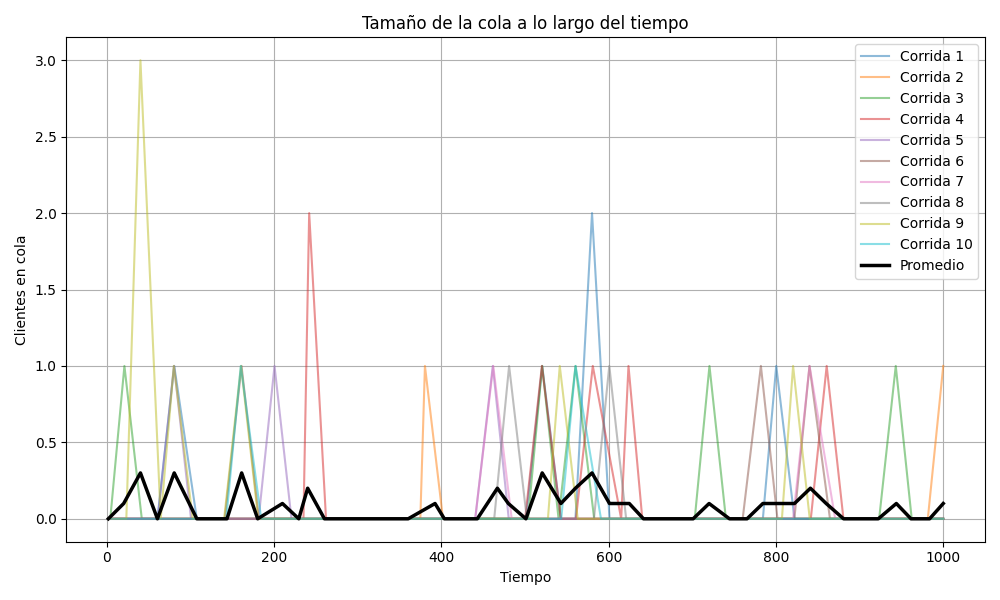
\includegraphics[width=0.8\textwidth]{Imagenes/MM1/cola_vs_tiempo_0.25_infinita.png}
        \caption{\( \lambda \) = 0.25: la cola casi no se forma, los clientes son muy infrecuentes, de 1 a 2 clientes, con promedio rozando cero.}
        \label{fig:ejemplo}
    \end{figure}
    \begin{figure}[h!]
        \centering
        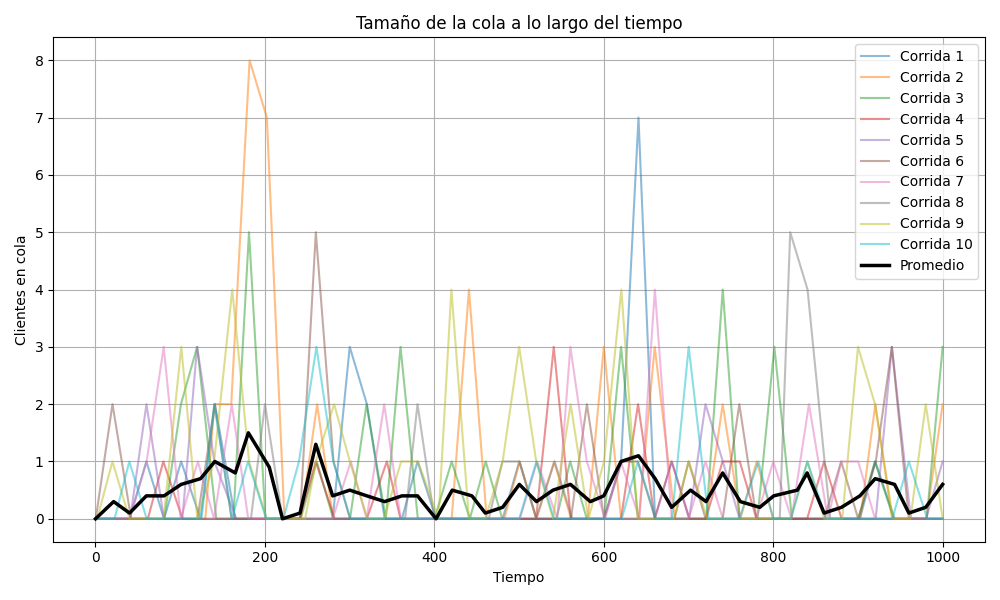
\includegraphics[width=0.8\textwidth]{Imagenes/MM1/cola_vs_tiempo_0.5_infinita.png}
        \caption{\( \lambda \) = 0.50:  el sistema casi siempre vacío o con máximo 2 a 3 clientes, promedio bajo, casi siempre cercano a cero.}
        \label{fig:ejemplo}
    \end{figure}
    \begin{figure}[h!]
        \centering
        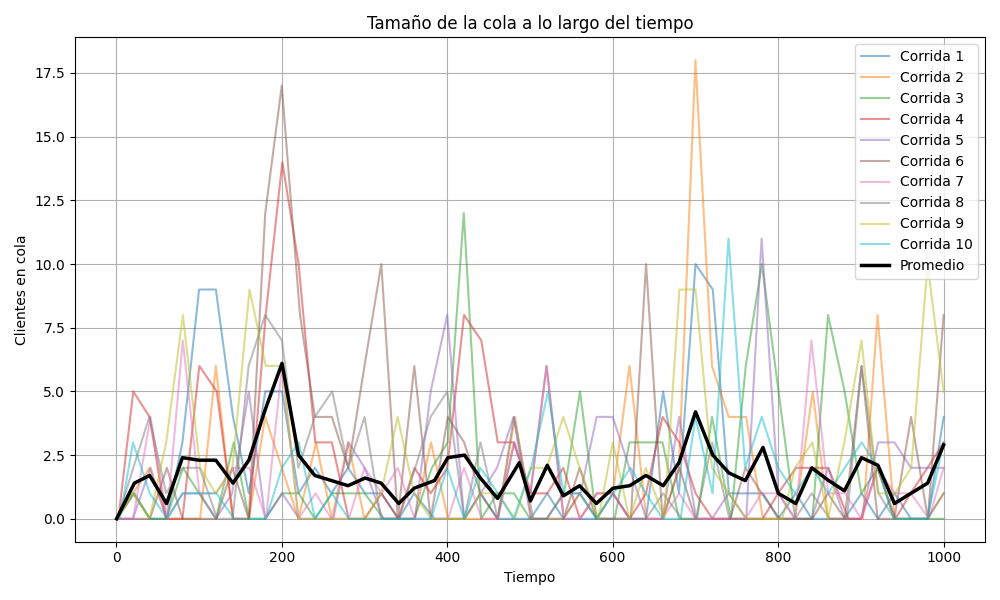
\includegraphics[width=0.8\textwidth]{Imagenes/MM1/cola_vs_tiempo_0.75_infinita.png}
        \caption{\( \lambda \) = 0.75: la cola fluctúa normalmente, con pocas acumulaciones, el promedio se mantiene estable entre 1 y 4 clientes.}
        \label{fig:ejemplo}
    \end{figure}

    \begin{figure}[h!]
        \centering
        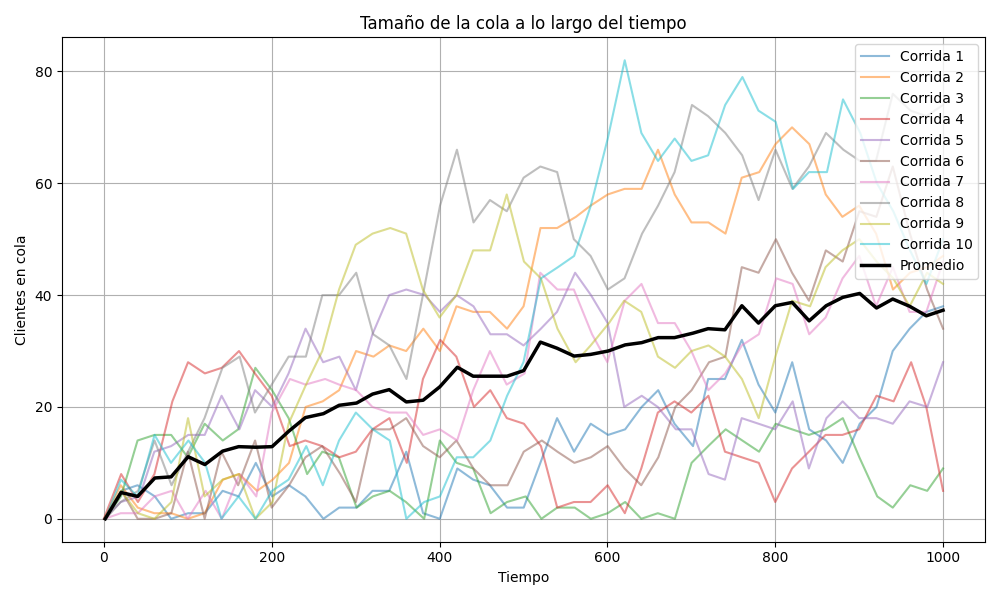
\includegraphics[width=0.8\textwidth]{Imagenes/MM1/cola_vs_tiempo_1.0_infinita.png}
        \caption{\( \lambda \) = 1: la cola casi no se forma, los clientes son muy infrecuentes, de 1 a 2 clientes, con promedio rozando cero.}
        \label{fig:ejemplo}
    \end{figure}
    
    \begin{figure}[h!]
        \centering
        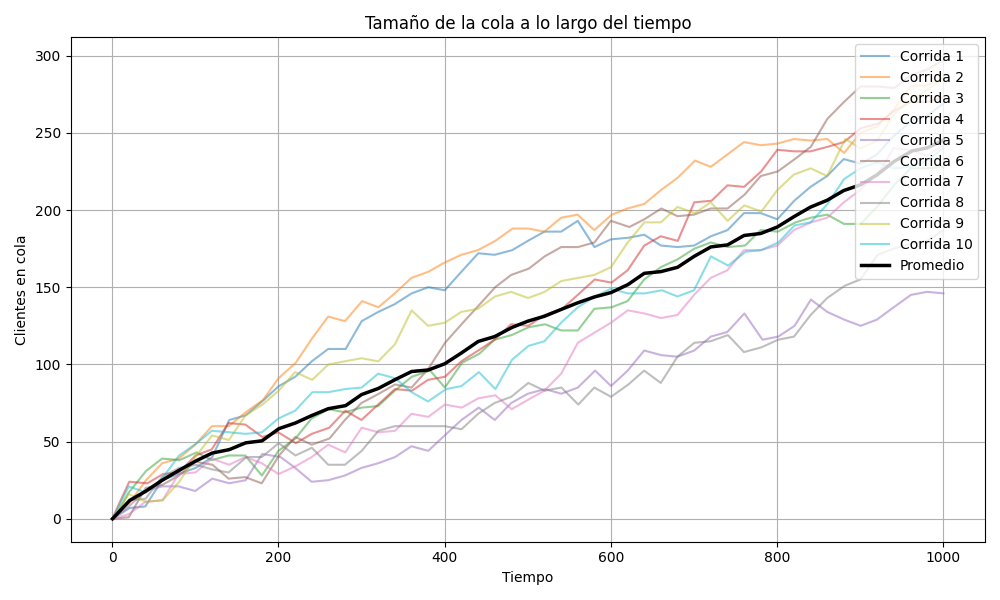
\includegraphics[width=0.8\textwidth]{Imagenes/MM1/cola_vs_tiempo_1.25_infinita.png}
        \caption{\( \lambda \) = 1.25:  la cola explota linealmente, con picos de hasta 300, promedio sube fuertemente, indicando inestabilidad total.}
        \label{fig:ejemplo}
    \end{figure}
\FloatBarrier

2- Cola vs Tiempo segun tasa de arribo  \( \lambda \) = 0,75, variando K finitos:

\begin{figure}
    \centering
    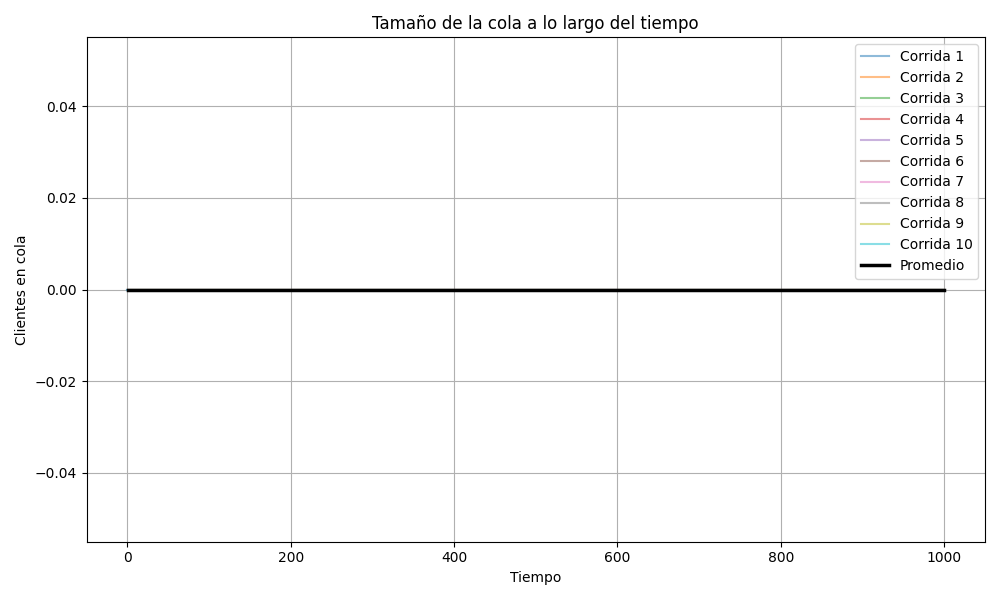
\includegraphics[width=0.5\linewidth]{Imagenes/MM1/cola_vs_tiempo_0.75_K0.png}
    \caption{K=0: nunca hay cola, la gráfica es plana en cero.}
    \label{fig:enter-label}
\end{figure}
\begin{figure}
    \centering
    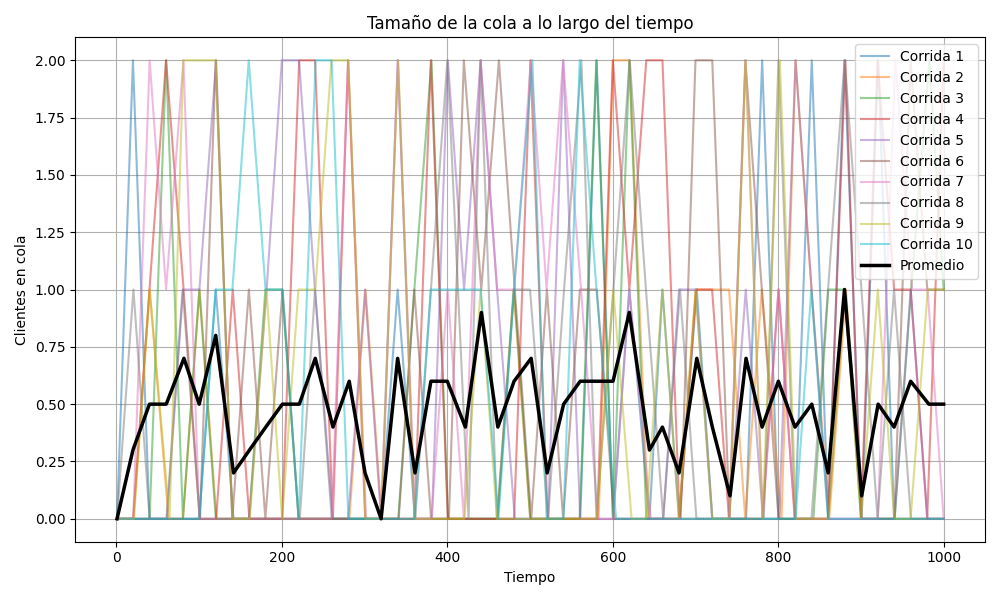
\includegraphics[width=0.5\linewidth]{Imagenes/MM1/cola_vs_tiempo_0.75_K2.png}
    \caption{K=2:la cola se mantiene entre 0 y 2, promedio estable entre 0.5‑0.9, pocas acumulaciones.}
    \label{fig:enter-label}
\end{figure}
\begin{figure}
    \centering
    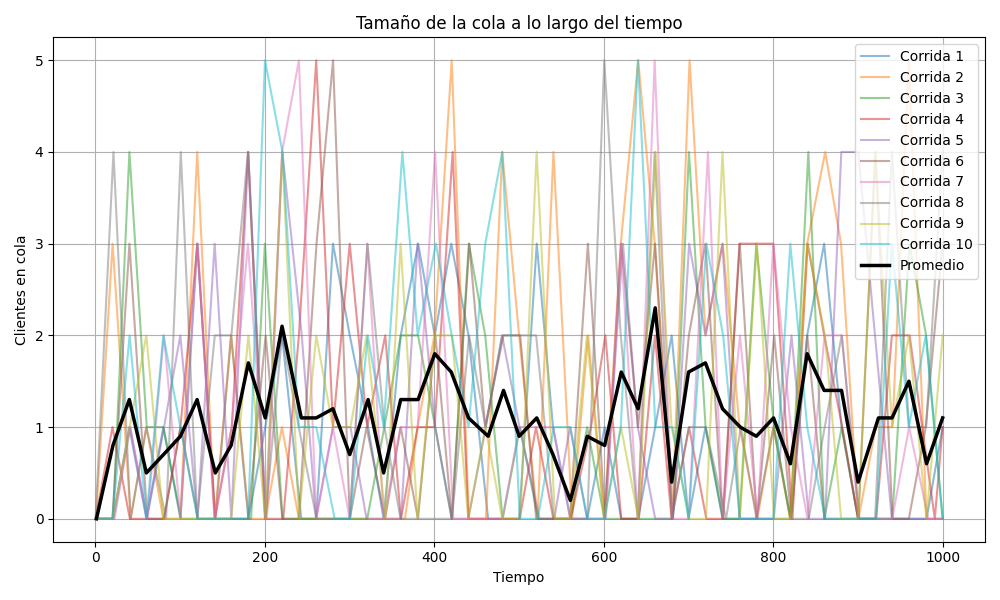
\includegraphics[width=0.5\linewidth]{Imagenes/MM1/cola_vs_tiempo_0.75_K5.png}
    \caption{K=5: la cola fluctúa entre 0‑5, promedio aparece entre 1 y 2, cortes por bloqueos ocasionales.}
    \label{fig:enter-label}
\end{figure}
\begin{figure}
    \centering
    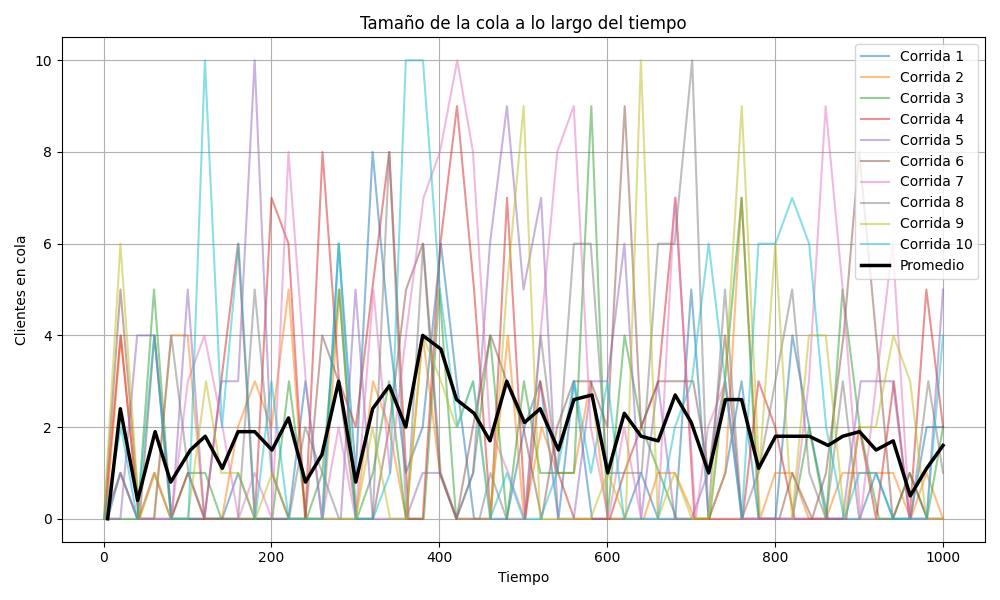
\includegraphics[width=0.5\linewidth]{Imagenes/MM1/cola_vs_tiempo_0.75_K10.png}
    \caption{K=10: permite hasta 10 clientes en cola, se observa variabilidad dispersa, promedio alrededor de 2, cortes por pérdidas cuando llena.}
    \label{fig:enter-label}
\end{figure}
\begin{figure}
    \centering
    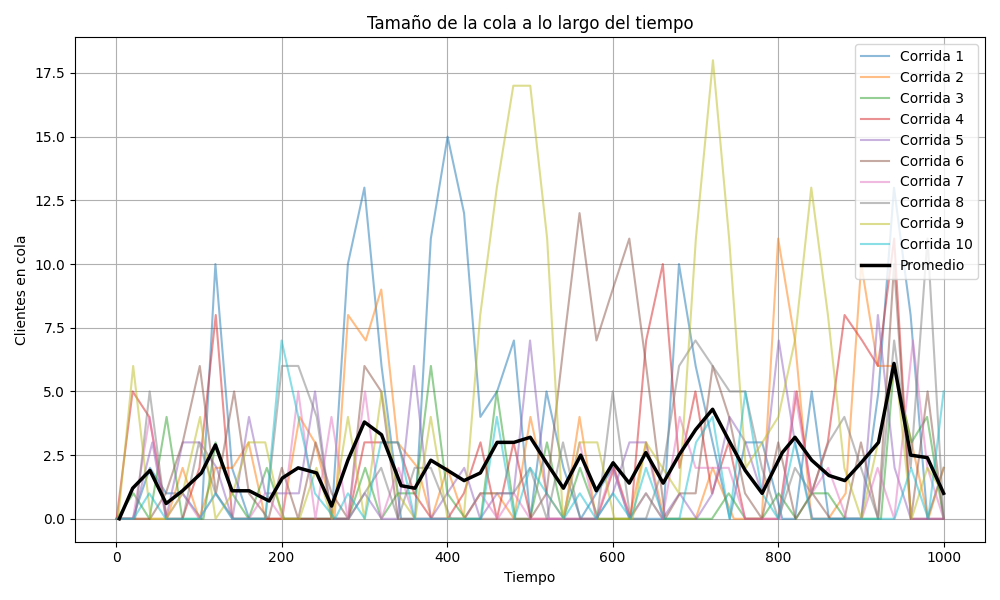
\includegraphics[width=0.5\linewidth]{Imagenes/MM1/cola_vs_tiempo_0.75_K50.png}
    \caption{K=50: varía considerablemente entre 10 simulaciones, aunque su promedio se mantiene generalmente bajo.}
    \label{fig:enter-label}
\end{figure}
\FloatBarrier

3- Probabilidad promedio de encontrar n clientes en cola: aqui hacemos una comparacion entre dos valores extremos, viendo como a mayor K se ve de manera más clara la distribucion exponencial, usando como ejemplo la tasa de arribo de 0.75.
\begin{figure}
    \centering
    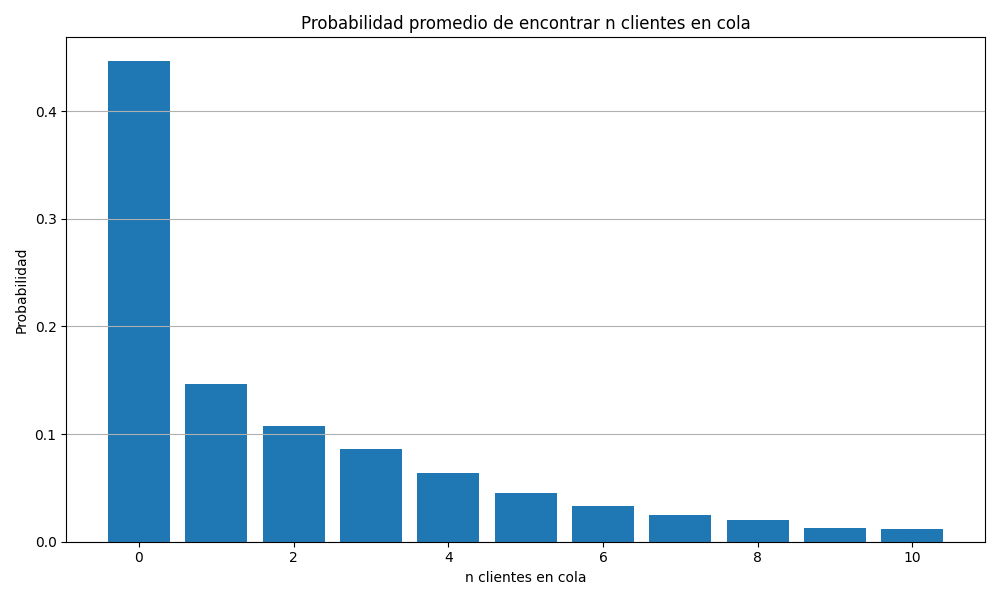
\includegraphics[width=0.5\linewidth]{Imagenes/MM1/prob_n_clientes_0.75_K10.png}
    \caption{K=10}
    \label{fig:enter-label}
\end{figure}
\begin{figure}
    \centering
    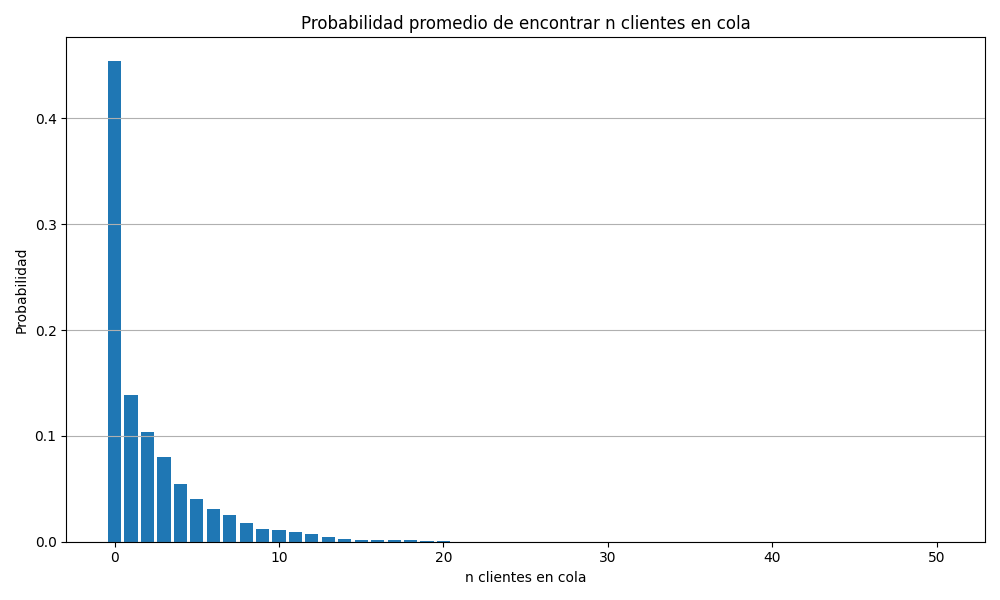
\includegraphics[width=0.5\linewidth]{Imagenes/MM1/prob_n_clientes_0.75_K50.png}
    \caption{K=50}
    \label{fig:enter-label}
\end{figure}
\FloatBarrier
Y ademas observamos como se llena la cola comparando las tasas de arribo, siendo la última de 1.25 la que colapsa el sistema, encontrándose la mayor probabilidad por encima de los 100 clientes.
\begin{figure}
    \centering
    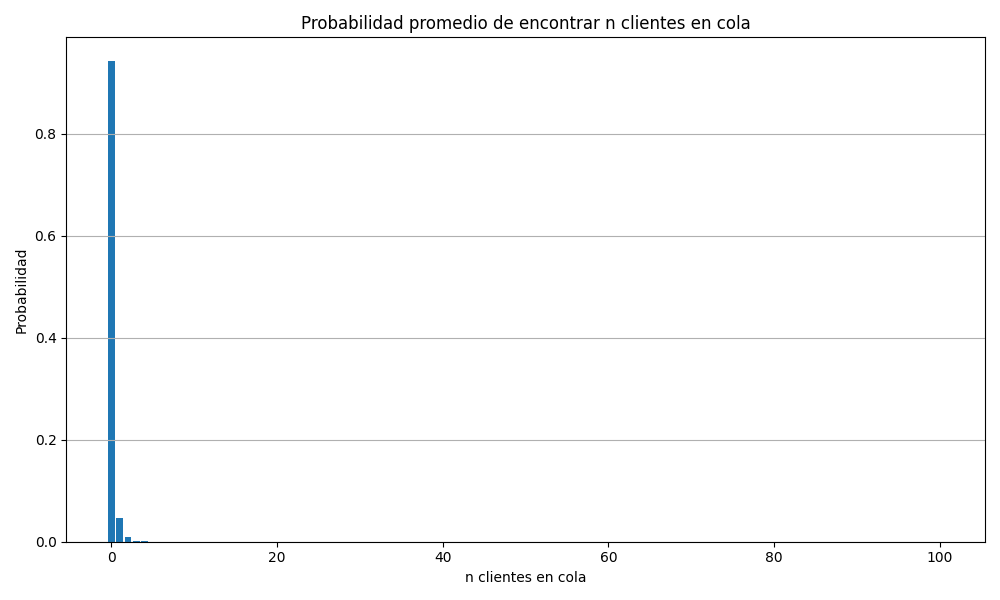
\includegraphics[width=0.5\linewidth]{Imagenes/MM1/prob_n_clientes_0.25_infinita.png}
    \caption{\( \lambda \)=0.25, K infinito}
    \label{fig:enter-label}
\end{figure}
\begin{figure}
    \centering
    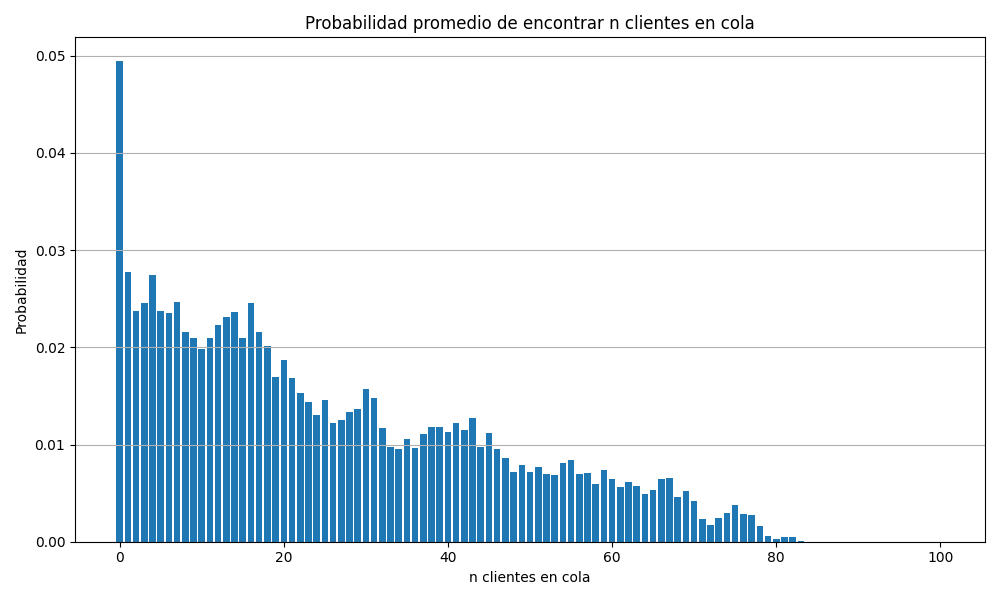
\includegraphics[width=0.5\linewidth]{Imagenes/MM1/prob_n_clientes_1.0_infinita.png}
    \caption{\( \lambda \)=1, K infinito}
    \label{fig:enter-label}
\end{figure}
\begin{figure}
    \centering
    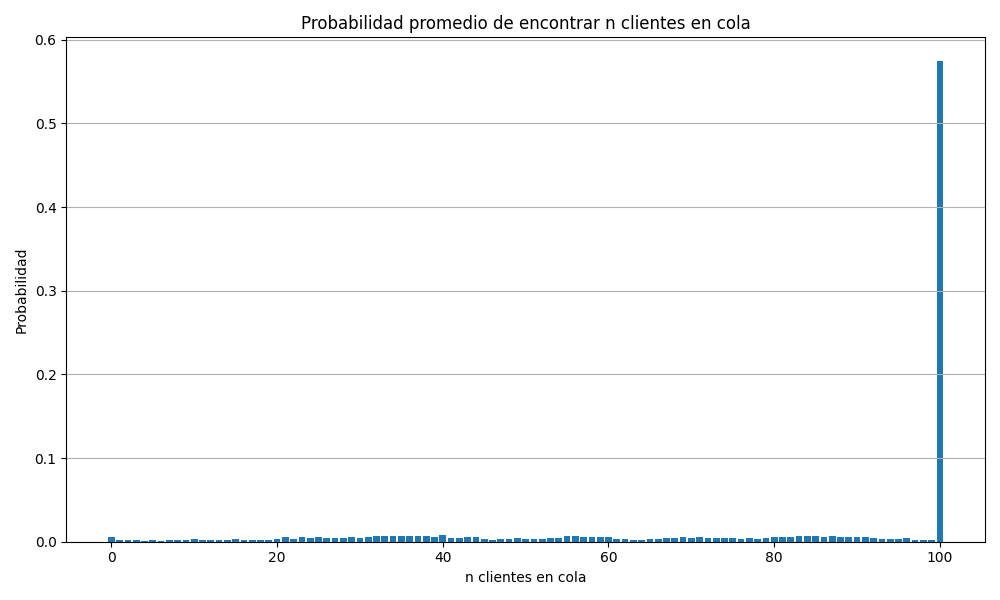
\includegraphics[width=0.5\linewidth]{Imagenes/MM1/prob_n_clientes_1.25_infinita.png}
    \caption{\( \lambda \)=1.25, K infinito}
    \label{fig:enter-label}
\end{figure}
\FloatBarrier

4- Utilizacion del servidor por corrida: aqui vemos como no conviene tener baja tasa de arribo para que el servidor no este oscioso, pero tampoco viene bien explotarlo ya que la cola no para de crecer. 
\begin{figure}
    \centering
    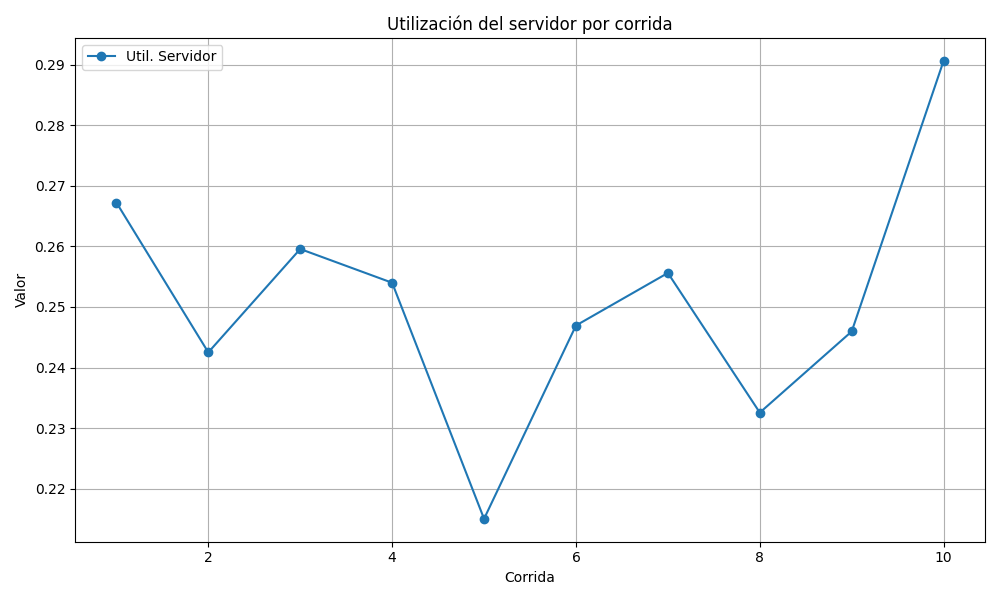
\includegraphics[width=0.5\linewidth]{Imagenes/MM1/util_sv_0.25_infinita.png}
    \caption{\( \lambda \)=0.25: la utilización del servidor es consistentemente baja, oscilando entre aproximadamente 0.21 y 0.29}
    \label{fig:enter-label}
\end{figure}
\begin{figure}
    \centering
    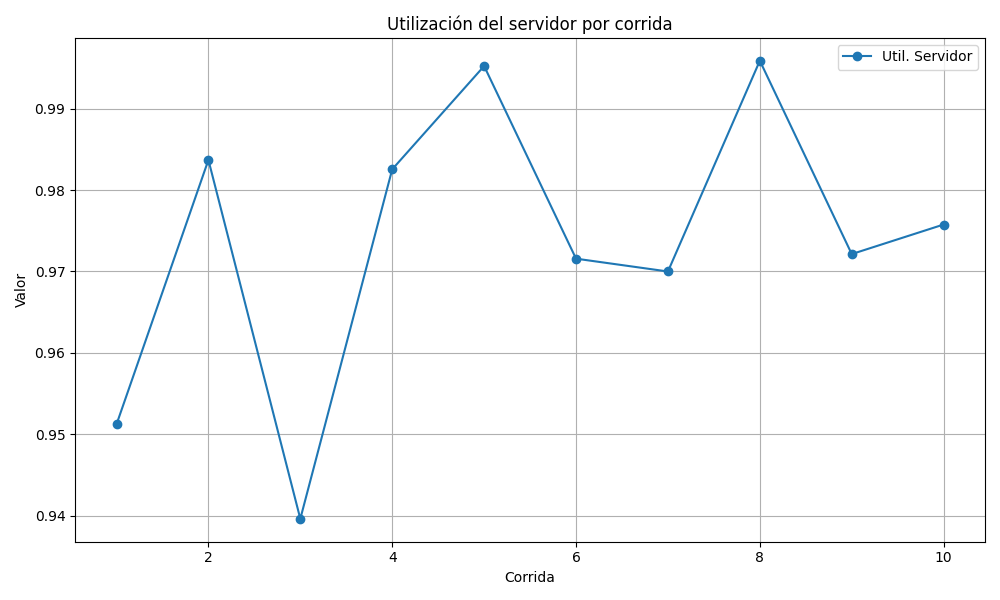
\includegraphics[width=0.5\linewidth]{Imagenes/MM1/util_sv_1.0_infinita.png}
    \caption{\( \lambda \)=1: la utilización del servidor se encuentra en un rango mucho más alto, mayormente por encima de 0.94, con picos cercanos a 0.99}
    \label{fig:enter-label}
\end{figure}
\begin{figure}
    \centering
    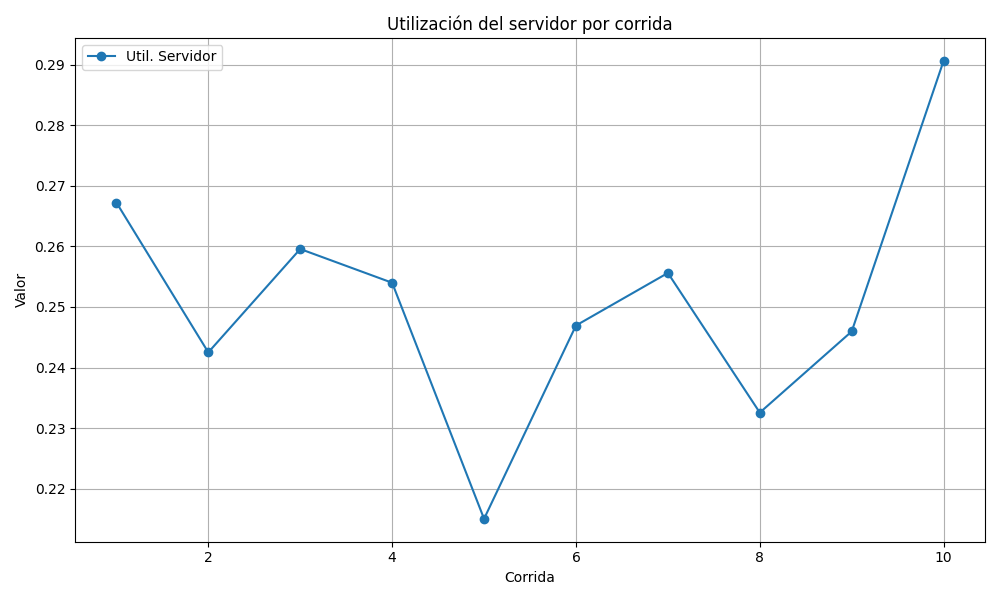
\includegraphics[width=0.5\linewidth]{Imagenes/MM1/util_sv_0.25_infinita.png}
    \caption{\( \lambda \)=1.25: La utilización del servidor es extremadamente alta y consistentemente cercana al 100 porciento (valores entre 0.993 y 0.999)}
    \label{fig:enter-label}
\end{figure}
\FloatBarrier

\subsection{En Anylogic}
...

\section{Modelo Inventario}

\subsection{Valor teorico esperado}

En el modelo de control de inventarios \((s, S)\), es posible estimar teóricamente el desempeño del sistema a través de ciertos valores esperados, como el nivel promedio de inventario y el costo total promedio. Estos valores dependen de la política adoptada, la distribución de la demanda y el tiempo de entrega.

Inventario promedio esperado:

\[
\mathbb{E}[I] = \frac{\text{Área bajo la curva del inventario a lo largo del tiempo}}{\text{Tiempo total}}
\]

Este valor representa el inventario promedio mantenido durante el tiempo y es afectado por los parámetros \(s\), \(S\), la distribución de la demanda y el lead time.

Costo total promedio esperado por unidad de tiempo:

\[
\mathbb{E}[C] = C_{\text{orden}} \cdot \frac{D}{Q} + C_{\text{mant}} \cdot \mathbb{E}[I] + C_{\text{faltante}} \cdot \mathbb{E}[B]
\]

Donde:
\begin{itemize}
    \item \(D\): demanda promedio por unidad de tiempo,
    \item \(Q = S - s\): tamaño del pedido,
    \item \(C_{\text{orden}}\): costo fijo por cada orden realizada,
    \item \(C_{\text{mant}}\): costo por mantener una unidad en inventario por unidad de tiempo,
    \item \(C_{\text{faltante}}\): costo por unidad en falta,
    \item \(\mathbb{E}[I]\): inventario promedio esperado,
    \item \(\mathbb{E}[B]\): valor esperado del número de unidades en falta.
\end{itemize}


\subsection{En Python}
Hicimos una simulación discreta en Python basada en el modelo clásico \((s, S)\). Este modelo establece que, cuando el nivel de inventario cae por debajo de un punto crítico \( s \), se realiza un pedido para reponer stock hasta alcanzar el nivel \( S \). La simulación permite analizar distintas combinaciones de políticas y tasas de demanda para observar su impacto en los costos del sistema.

El programa está organizado en torno a una estructura de eventos discretos, donde los eventos se gestionan mediante una cola de prioridad, utilizando el módulo `heapq`. Los eventos considerados son:

\begin{itemize}
    \item La llegada de un pedido proveniente del proveedor.
    \item Una demanda de un cliente.
    \item La evaluación mensual del nivel de inventario.
    \item El fin de la simulación (tras un año).
\end{itemize} 

Los parámetros clave del modelo se reciben por línea de comandos, lo que permite ejecutar fácilmente múltiples pruebas con diferentes configuraciones. Entre ellos se encuentran los niveles \( s \) y \( S \), y el tiempo promedio entre demandas.

El nivel inicial de inventario se establece en \( S \), y se asume que la simulación tiene una duración de 12 meses. Durante ese período, las demandas se generan aleatoriamente siguiendo una distribución discreta con pesos definidos, representando tamaños posibles de pedido de los clientes (por ejemplo, entre 1 y 5 unidades).

Cada vez que ocurre una demanda, el inventario se reduce en función del tamaño solicitado. Si, al evaluar el inventario a comienzos de cada mes, el nivel es menor que \( s \) y no hay pedidos en curso, se genera un nuevo pedido cuya llegada se programará con un retraso aleatorio entre 0.5 y 1.0 meses.

Como ya dijimos, el sistema considera distintos tipos de costos:

\begin{itemize}
    \item Costo de orden: compuesto por un valor fijo y un costo incremental por unidad pedida.
    \item Costo de mantenimiento: proporcional al inventario positivo promedio.
    \item Costo por faltante: proporcional al inventario negativo promedio (cuando no se puede satisfacer la demanda).
\end{itemize}

Durante la simulación, se lleva un registro continuo del nivel de inventario a intervalos regulares (cada 0.1 meses), lo cual permite generar gráficos de comportamiento a futuro. Finalizada cada corrida, se calculan los costos acumulados y promedios, y se almacenan en un archivo CSV junto con los niveles de inventario a lo largo del tiempo.

Se realizaron 10 corridas para cada política, con el objetivo de reducir la variabilidad inherente a la simulación estocástica y obtener valores representativos.

\subsubsection{Graficas de comparacion en 10 corridas}
1- Nivel de inventario a lo largo del tiempo
\begin{figure}
    \centering
    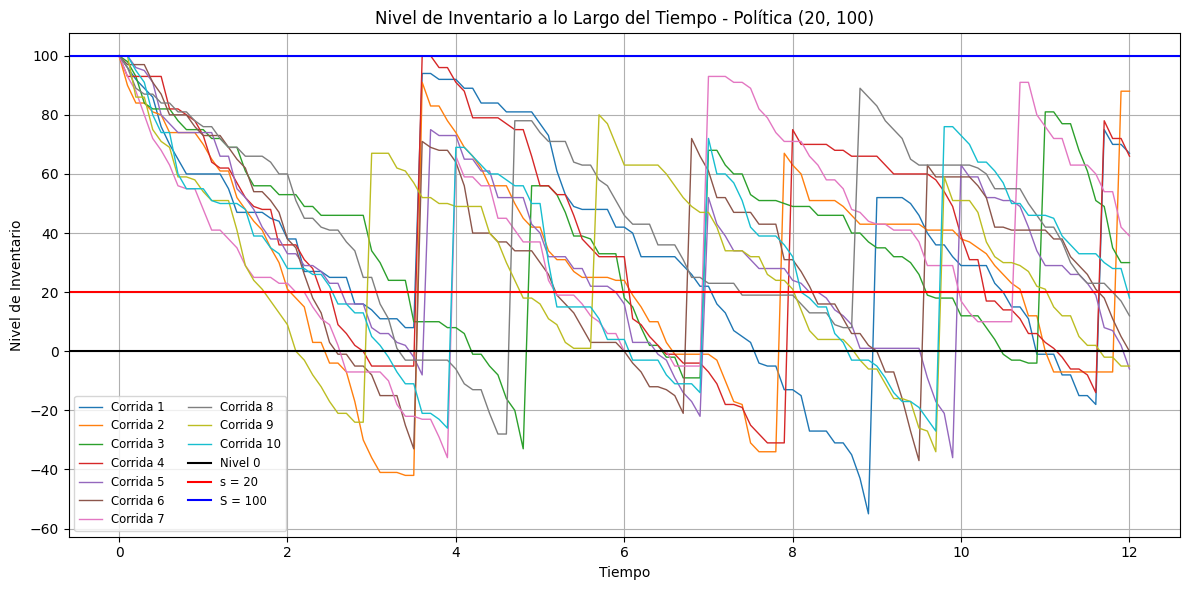
\includegraphics[width=0.5\linewidth]{Imagenes/Inventario/inventario_vs_tiempo_20_100.png}
    \caption{esta politica muestra fluctuaciones y deficits}
    \label{fig:enter-label}
\end{figure}
\FloatBarrier
2- Promedios según la politica (20,100)
\begin{figure}
    \centering
    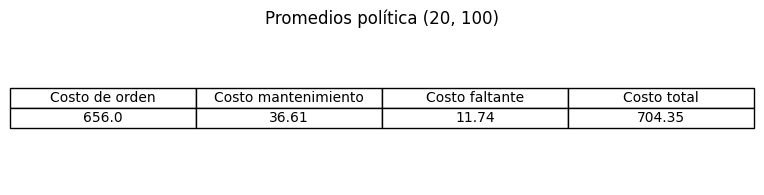
\includegraphics[width=0.5\linewidth]{Imagenes/Inventario/promedios_20_100.png}
    \caption{Promedios asociados a esta politica}
    \label{fig:enter-label}
\end{figure}
\FloatBarrier

\subsection{En Anylogic}


\section{Conclusiones}

veremos...





\bibliographystyle{unsrt}  
\begin{thebibliography}{2}

\bibitem{simulaciongithub}
Aldana Risso Patrón. \textit{TP 3 - Simulación de modelos: MM1 e Inventario (código fuente)}.\\
Disponible en: \url{https://github.com/AldanaRP/TPSimulacion} \\

\bibitem{bacchini2018}
Bacchini, H. \textit{Introducción a la Probabilidad y a la Estadística}.\\
Universidad de Buenos Aires, Facultad de Ciencias Económicas, 2018.\\
Disponible en: \url{http://bibliotecadigital.econ.uba.ar/download/libros/Bacchini_Introduccion-a-la-probabilidad-y-a-la-estadistica-2018.pdf}\\

\bibitem{libro}
Averill M. Law \textit{Simulation modeling and analysis. Fifth edition }2015. \\
Disponible en:
\url{https://drive.google.com/file/d/1ycmnW5F-kY06XxyGKrjpVFNETkTKkBUV/view}

\end{thebibliography}

\end{document}
